\documentclass[ngerman]{report}
\usepackage{graphicx}
\usepackage[german,ngerman]{babel}
\title{SWPP Zusammenfassung}
    \author{Emanuel Gstrein, Felix Riml, Raphael Walter}
    \begin{document}
    \maketitle

    \newpage
    \tableofcontents
    \newpage

    \section{Definition}
    Das Projekt zielt darauf ab, eine Anwendung zu entwickeln, die Benutzern hilft, ihre Ausgaben in verschiedenen Währungen zu verwalten und in Echtzeit in ihre Heimatwährung umzurechnen. 
    Die Anwendung ermöglicht es, Ausgaben in mehreren Währungen einzugeben, diese kategorisch zu verwalten und die aktuellen Wechselkurse über eine API abzurufen. Zudem wird eine grafische 
    Übersicht über die Ausgaben geboten, um den Nutzern zu helfen, ihre finanziellen Aktivitäten besser zu verstehen und zu steuern.
    
    \section{Zielsetzung (SMART)}
    Das Ziel des Projekts ist es, innerhalb dieses Schuljahres
    eine voll funktionsfähige Anwendung zu entwickeln,
    die es Benutzern ermöglicht, ihre Ausgaben zu verfolgen
    und in Echtzeit zwischen verschiedenen Währungen zu konvertieren.
    Der Erfolg wird daran gemessen, dass mindestens 50 Benutzer
    die Anwendung innerhalb von drei Monaten nach der Veröffentlichung
    aktiv nutzen und mindestens 80 Prozent von ihnen angeben, dass sie die
    Anwendung hilfreich finden, um ihre Finanzen zu verwalten.
    Die Anwendung wird zudem eine benutzerfreundliche Oberfläche
    und eine klare Darstellung der Ausgaben in Form von Diagrammen bieten,
    um die Nutzererfahrung zu verbessern.

    \section{Projektorganisation}
    \subsection{Beteiligte Personen}
    \begin{itemize}
        \item Projektauftraggeber: Schule
        \item Projektleiter: Felix
        \item Projektmitarbeiter: Emanuel, Raphael
        \item Kunde: Endbenutzer
    \end{itemize}

    \section{Projektablaufplan}
    \subsection{Zweck und Ziel}
    Der Projektablaufplan dient zur Übersicht und Organisation aller 
    Projektaufgaben und -phasen. Er strukturiert die Aufgaben und ihre 
    Zusammenhänge klar und übersichtlich. Abbldung \ref{fig:Abbildung 1} zeigt die Planung des Gantt-Diagrams.
    In Abbildung \ref{fig:Abbildung 2} ist das Gantt-Diagramm zu sehen.

    \begin{figure}[h]
        \centering
        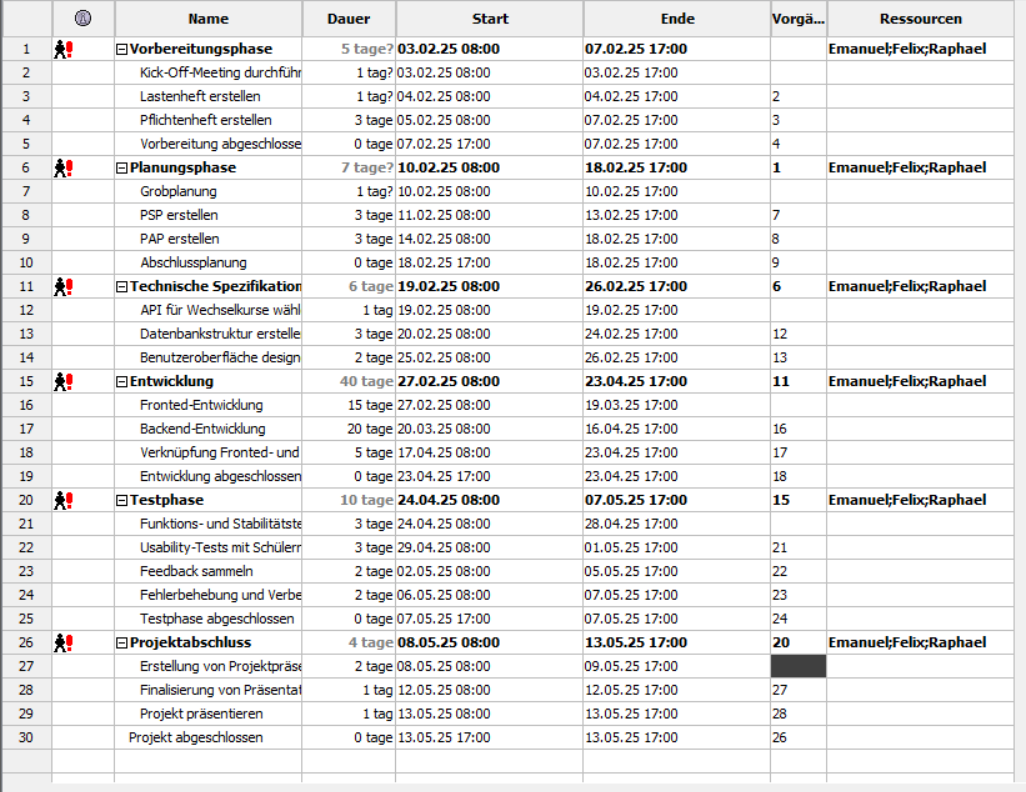
\includegraphics[width=0.8\textwidth]{images/Gantt1.png}
        \caption{Planung des Ganntt-Diagrams durch Projektlibre}
        \label{fig:Abbildung 1}
    \end{figure}
        
    \begin{figure}[h]
        \centering
        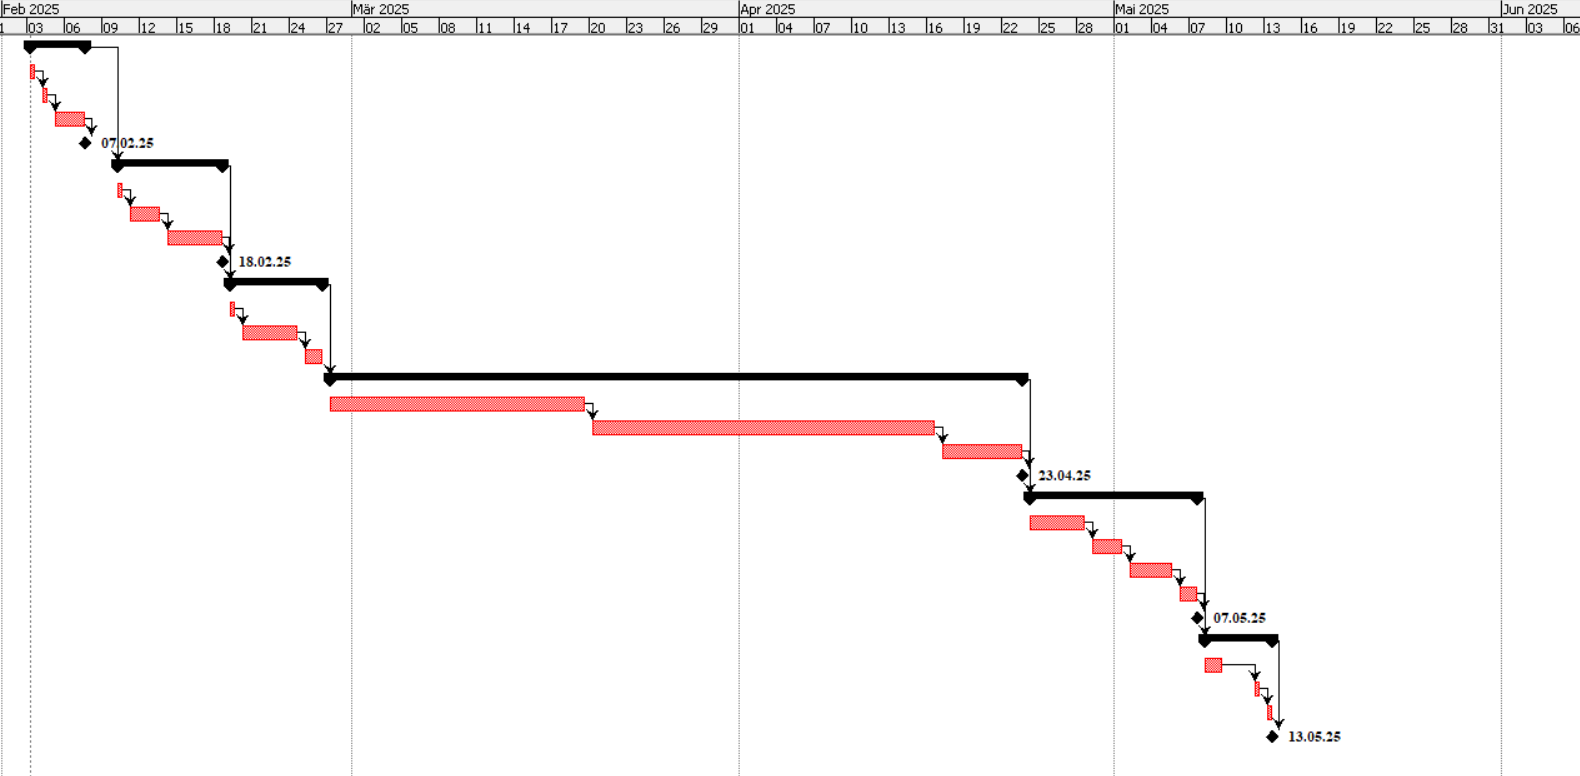
\includegraphics[width=0.8\textwidth]{images/Gantt2.png}
        \caption{Gantt-Diagramm}
        \label{fig:Abbildung 2}
    \end{figure}

    


 
\end{document}